%%%%%%%%%%%%%%%%%%%%%%%%%%%%%%%%%%%%%
%                                   %
% Compile with XeLaTeX and biber    %
%                                   %
% Questions or comments:            %
%                                   %
% joshua dot mcneill at uga dot edu %
%                                   %
%%%%%%%%%%%%%%%%%%%%%%%%%%%%%%%%%%%%%

\documentclass{beamer}
  % Read in standard preamble (cosmetic stuff)
  %%%%%%%%%%%%%%%%%%%%%%%%%%%%%%%%%%%%%%%%%%%%%%%%%%%%%%%%%%%%%%%%
% This is a standard preamble used in for all slide documents. %
% It basically contains cosmetic settings.                     %
%                                                              %
% Joshua McNeill                                               %
% joshua dot mcneill at uga dot edu                            %
%%%%%%%%%%%%%%%%%%%%%%%%%%%%%%%%%%%%%%%%%%%%%%%%%%%%%%%%%%%%%%%%

% Beamer settings
% \usetheme{Berkeley}
\usetheme{CambridgeUS}
% \usecolortheme{dove}
% \usecolortheme{rose}
\usecolortheme{seagull}
\usefonttheme{professionalfonts}
\usefonttheme{serif}
\setbeamertemplate{bibliography item}{}

% Packages and settings
\usepackage{fontspec}
  \setmainfont{Charis SIL}
\usepackage{hyperref}
  \hypersetup{colorlinks=true,
              allcolors=blue}
\usepackage{graphicx}
  \graphicspath{{../../figures/}}
\usepackage[normalem]{ulem}
\usepackage{enumerate}

% Document information
\author{M. McNeill}
\title[FREN2001]{Français 2001}
\institute{\url{joshua.mcneill@uga.edu}}
\date{}

%% Custom commands
% Lexical items
\newcommand{\lexi}[1]{\textit{#1}}
% Gloss
\newcommand{\gloss}[1]{`#1'}
\newcommand{\tinygloss}[1]{{\tiny`#1'}}
% Orthographic representations
\newcommand{\orth}[1]{$\langle$#1$\rangle$}
% Utterances (pragmatics)
\newcommand{\uttr}[1]{`#1'}
% Sentences (pragmatics)
\newcommand{\sent}[1]{\textit{#1}}
% Base dir for definitions
\newcommand{\defs}{../definitions}


  % Packages and settings

  % Document information
  \subtitle[Pronoms compléments d'objet]{D'autres pronoms compléments d'objet}

\begin{document}
  % Read in the standard intro slides (title page and table of contents)
  \begin{frame}
    \titlepage
    \tiny{Office: % Basically a variable for office hours location
Gilbert 121\\
          Office hours: % Basically a variable for office hours
 lundi, mercredi, vendredi 10:10--11:10
}
  \end{frame}

  \begin{frame}{L'ordre des pronoms}
    \centering
    \begin{tabular}{l | l | l | l}
      \parbox{0.2\linewidth}{Objet direct\\OU indirect} & Objet direct & Objet indirect & Autre \\
      \hline
      me                                                & le           & lui          & en \\
      te                                                & la           & leur         & \\
      nous                                              & les          &              & \\
      vous                                              &              &              & \\
    \end{tabular}

    \vspace{0.5cm}
    L'ordre suit \gloss{follows} le nombre de pronoms dans la catégorie.
  \end{frame}

  \begin{frame}[t]{Au bord du lac}{}
    \begin{center}
      {\tiny Un dimanche après-midi à l'île de la Grande Jatte (1884-1886) - Georges Seurat}
      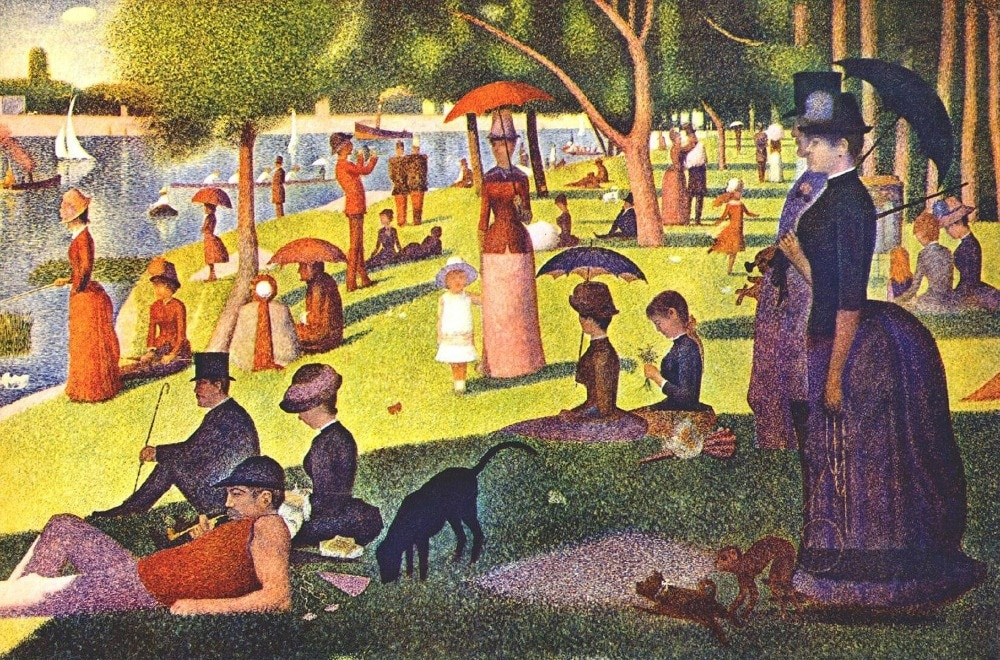
\includegraphics[scale=0.18]{dimanche_parc.jpg}
    \end{center}
    {\small
    Béa dit:
    \begin{itemize}
      \only<1-2>{
        \item Paul voit \textcolor{red}{ma sœur et moi} au bord du lac.
        \item<2> Paul \textcolor{red}{nous} voit au bord du lac.}
      \only<3-4>{
        \item Il téléphone \textcolor{blue}{à elle} parce qu'il est étrange.
        \item<4> Il \textcolor{blue}{lui} téléphone parce qu'il est étrange.}
      \only<5-6>{
        \item Le chien de Paul renifle \gloss{sniffs} \textcolor{red}{moi}.
        \item<6> Le chien de Paul \textcolor{red}{me} renifle.}
      \only<7-8>{
        \item Soudain, le chien donne \textcolor{red}{l'oiseau dans sa bouche} \textcolor{blue}{à moi}.
        \item<8> Soudain, le chien \textcolor{blue}{me} \textcolor{red}{le} donne.}
    \end{itemize}}
  \end{frame}

  \begin{frame}{}
    \begin{center}
      \Large Quiz
    \end{center}
  \end{frame}

  \begin{frame}{Invite-les!}
    \small
    \begin{enumerate}
      \item Écris une liste de trois activités que tu veux faire (surtout les activités sur la page 264!).
      \item Ensuite, pour chaque activité, trouve trois personnes dans la classe qui aimeraient faire \gloss{would like to do} ces activités avec toi.
      \item Si on accepte, détermine le jour et l'heure du rendez-vous.
      \item Écris leurs noms pour te les rappeler.
      \item Si un/e camarade de classe t'invite à faire une activité, tu peux refuser ou accepter selon tes intérêts \gloss{your interests}.
    \end{enumerate}
    \begin{description}
      \item[] \textbf{Modèle:}
      \item[E1:] Je veux faire un pique-nique. Est-ce que tu veux m'accompagner?
      \item[E2:] D'accord! Où est-ce qu'on va se retrouver?
      \item[E1:] Dans le parc Bishop. Est-ce que tu vas être libre demain à 11h?
      \item[E2:] Oui! Je vais être libre.
    \end{description}
  \end{frame}

  \begin{frame}{}
    \begin{center}
      \Large Questions?
    \end{center}
  \end{frame}
\end{document}
